\documentclass[a4paper,
12pt,
BCOR12mm,
]{scrartcl}
%scrreport
\usepackage[ngerman]{babel}
\usepackage[utf8]{inputenc}
\usepackage[T1]{fontenc}
\usepackage{url}
\usepackage{graphicx}
\title{APUVS, Blatt 2}
\author{Jan Fajerski and Kai Warncke and Magnus Müller}

\begin{document}
\maketitle  

\section*{Aufgabe 2.1}
  \subsection*{Testumgebung}
    Die Tests wurden lokal auf einem Thinkpad T410 mit Intel i5 M520 @ 2,4GHz und 4 GB Arbeitsspeicher durchgeführt.
    Im Netzwerk wurde auf dem Thinkpad T410 und einem Thinkpad T500 mit Intel Core2 Duo @ 2,53GHz und 4GB Arbeitsspeicher über das Eduroam Wlan
    an der HU gearbeitet.
  \subsection*{Testergebnisse}
{\scriptsize
\begin{tabular}[10pt]{|p{3cm}|p{3cm}|p{3cm}|p{3cm}|}
      \hline &&&\\
      Send-Typ                      & relativer Speedup $S_8$       & linearer Speedup  $S_8$       & Effizienz $E_8$   \\
      \hline &&&\\
      blockierendes Senden lokal    & 0.0512                        & 8                             & 0.00625           \\
      \hline &&&\\
      blockierendes Senden verteilt & 0.0077                        & 8                             & 0.00096           \\
      \hline &&&\\
      Standartsenden lokal          & 0.027                         & 8                             & 0.0033            \\
      \hline &&&\\
      Standartsenden verteilt       & 0.011                         & 8                             & 0.0013            \\
      \hline &&&\\
      Ready-Send lokal              & 0.027                         & 8                             & 0.0033            \\
      \hline &&&\\
      Ready-Send verteilt           & 0.0058                        & 8                             & 0.00072           \\
      \hline &&&\\
      synchrones Senden lokal       & 0.0326                        & 8                             & 0.00408           \\
      \hline &&&\\
      synchrones Senden verteilt    & 0.0118                        & 8                             & 0.00147           \\
      \hline 
    \end{tabular}}

\subsection*{Graphische Darstellung}
\subsubsection*{Laufzeitdiagramme}
	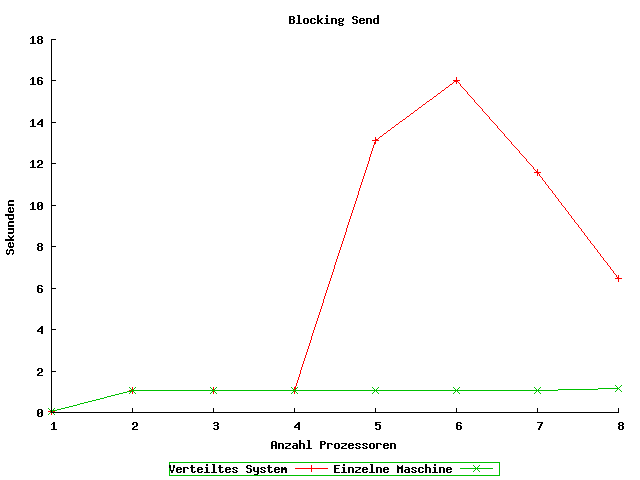
\includegraphics[width=0.5\linewidth]{../a_2_1/data/png/blockingsend.png}
	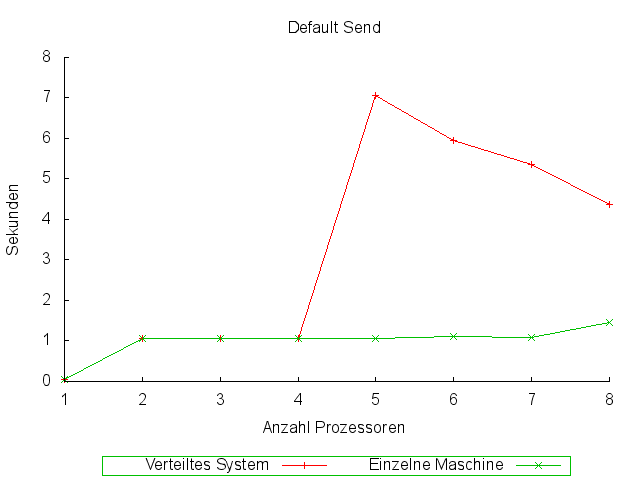
\includegraphics[width=0.5\linewidth]{../a_2_1/data/png/defaultsendtype.png}
	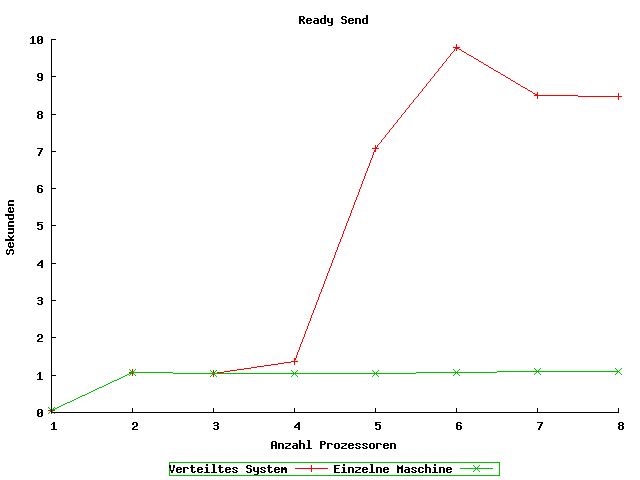
\includegraphics[width=0.5\linewidth]{../a_2_1/data/png/readysendtype.png}
	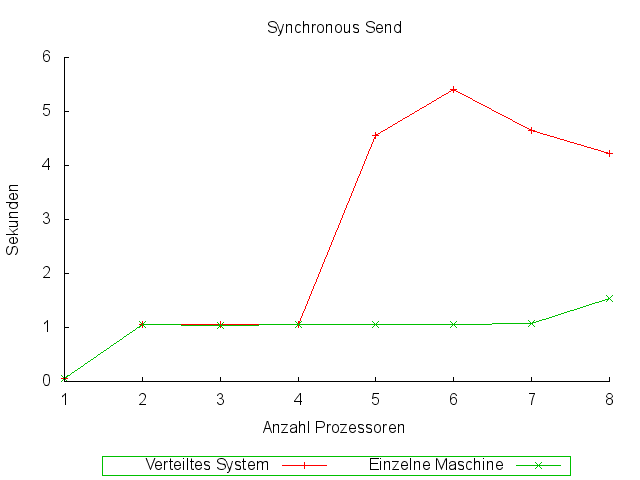
\includegraphics[width=0.5\linewidth]{../a_2_1/data/png/synchronsendtype.png}
\subsubsection*{Speedup-/Effizienzdiagramme}
	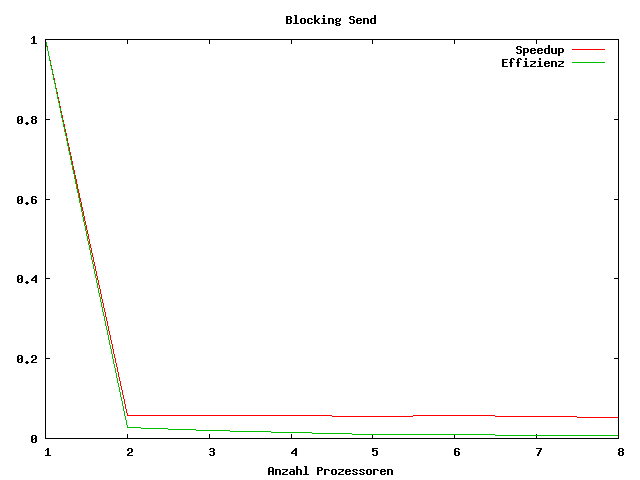
\includegraphics[width=0.5\linewidth]{../a_2_1/data/png/speed_eff_bs.png}
	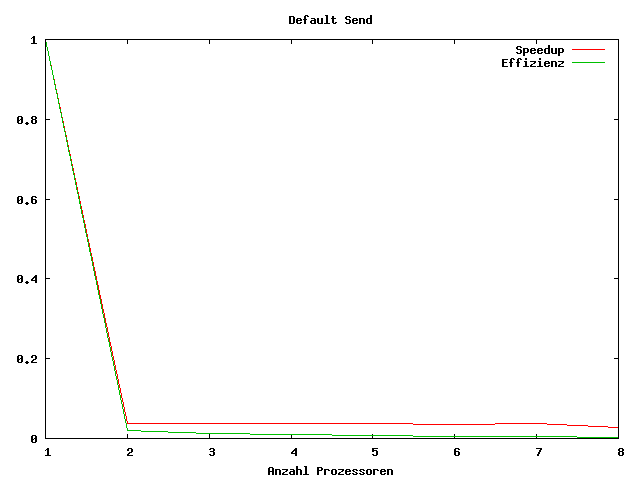
\includegraphics[width=0.5\linewidth]{../a_2_1/data/png/speed_eff_ds.png}
	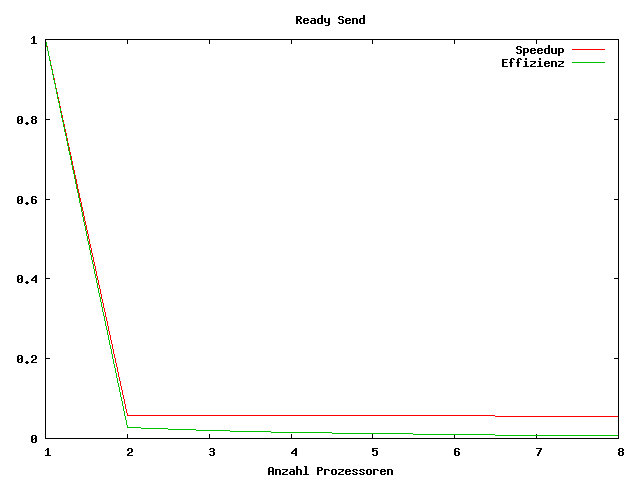
\includegraphics[width=0.5\linewidth]{../a_2_1/data/png/speed_eff_rs.png}
	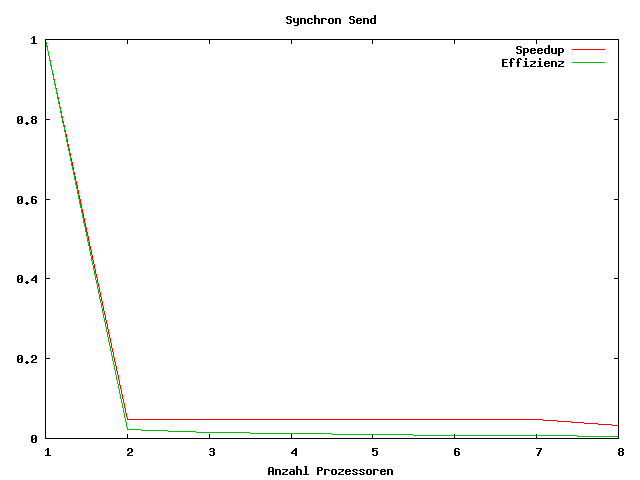
\includegraphics[width=0.5\linewidth]{../a_2_1/data/png/speed_eff_ss.png}
Aus den Laufzeit- sowie den Speedup-/Effizienzdiagrammen ist ein starker Slowdown zu erkennen wenn das Problem
auf mehreren PEs bearbeitet wird. Der Mehraufwand der Parallelisierung übersteigt klar den erreichten Gewinn. 


\section*{Aufgabe 2.2}
Laut \verb|$ man mpi_send| ist die Standardmethode zum Versenden von Nachrichten in
openmpi synchron und blockierend:
\begin{verbatim}
DESCRIPTION
	MPI_Send performs a standard-mode, blocking send.
\end{verbatim}

Laut dem Testprogramm \verb|send_block| scheint es jedoch eine gepufferte Version zu sein.



\section*{Aufgabe 2.4}
Zu den Hauptproblemen zählt:
\begin{itemize}
	\item verschiedene MPI Implementationen
	\item verschiedene Rechner-Architekturen
	\item verschiedene Dateisysteme
	\item die verschiedenen Knoten sind unter Umständen nicht immer erreichbar
\end{itemize}

Lösungsansätze:
\begin{itemize}
	\item Verwendung einer einheitlichen MPI-Implementation. Hierzu gehört auch die
		Verwendung der gleichen Version, denn verschiedene Versionen sind nicht zwingend
		ABI-kompatibel.
	\item Abstraktion weg von der unterliegenden Architektur. Ähnlich der OSI-Layer sollten
	die MPI-Implementationen die zugrunde liegende Architektur möglichst verbergen.
\end{itemize}

%\nocite{*}
%\bibliographystyle{alphadin}
%\bibliography{bibliography.bib}

\end{document}
